\chapter{Estado Del Arte}
\label{cap:estadoArte}

Uno de los primeros pasos para la creación de la aplicación VitHabitus ha sido analizar el mercado para poder entrar en sintonía con aquellas aplicaciones más populares. Esta investigación permite extraer ideas, modelos, interfaces, estructuras, componentes y mucha más información que facilitan enormemente el desarrollo de una aplicación competitiva para el mercado.

De esta manera, este capítulo recoge una revisión de varias de las aplicaciones más usadas relacionadas con el ámbito de la salud y de la planificación de hábitos, identificando tanto las fortalezas y debilidades de cada una, como las  características comunes que resultan esenciales para el atractivo de una aplicación.

Entre las aplicaciones que se analizaron se encuentran ``Habitify'', ``Quitzilla'', ``Way of life'', ``INDYA'', ``HabitNow'', ``Habitica'', ``Todoist''. 

A la hora de evaluar las aplicaciones se han seguido ciertos criterios y parámetros con el fin de obtener una visión crítica y equilibrada. En primer lugar, se ha analizado la experiencia de usuario, valorando la facilidad de navegación, la claridad de las instrucciones y explicaciones de uso y la fluidez general del recorrido de navegación. También se ha tenido en cuenta el diseño y los efectos visuales, examinando el atractivo estético, la calidad del diseño y la presentación visual. Siendo estos factores importantes para fomentar el compromiso del usuario hacia la aplicación.

Otro aspecto a considerar ha sido la flexibilidad de cada aplicación, evaluando su capacidad para adaptarse a circunstancias cambiantes, como la modificación de objetivos o la reprogramación de actividades de un día para otro. Surge también el término ``Gamificación'', básicamente consiste en examinar de que maneras la aplicación incorpora elementos de juego como recompensas, insignias o sistemas de rachas que motivan y atrapan a los usuarios a seguir consumiendo la aplicación. Se trata de un elemento interesante, que bien implementado tiene mucho éxito. 

En cuanto a componentes técnicos, muchas de estas aplicaciones se encuentran desplegadas en dispositivos móviles y en ordenadores, por lo que un factor importante para la escalabilidad es la diferencia de implementación entre los diferentes entornos (aunque de momento VitHabitus tiene como único objetivo los teléfonos móviles). 

Por último, se analizó la parte de comercialización. Todas estas aplicaciones que se analizarán a continuación, son de uso gratuito en una primera instancia, pero algo que también todas tienen en común, es la existencia de un plan superior al gratuito, el ``plan premium'',  en el cual a cambio de pagar una cuota mensual o anual, se ofrecen ciertos privilegios adicionales. En términos generales, se analizó el coste de esos planes de pago  y la relación calidad-precio entre servicios y coste. Además, muchas aplicaciones se apoyan en la premisa de ser aplicaciones gratuitas a pesar de que su plan gratuito cuenta con tantas restricciones que el usuario poco puede hacer en ella sin invertir en un plan superior.

\section{Habitica}

La primera de las aplicaciones a mencionar es Habitica. Se trata de una aplicación basada en la gestión de hábitos pero con un enfoque más interactivo y con juegos de rol. Mezcla la productividad con la diversión lo que lo convierte en una aplicación que combina a la perfección la tarea de gestión de hábitos y la retención del usuario.

\begin{figure}[h]
	\centering
	\includegraphics[width = 1\textwidth]{Imagenes/apps_images/habitica.png}
	\caption{Flujo de funcionamiento de Habitica}
	\label{fig:Habitica}
\end{figure}

Como aspectos a destacar, es necesaria la creación de una cuenta de usuario para poder acceder. Desde la pantalla de inicio explica de forma amena la finalidad de la aplicación para facilitar al usuario su integración con la aplicación. Una vez hecho el log-in, se presenta la pantalla de inicio en la cual se puede acceder a los distintos componentes y servicios de la aplicación. Para mayor inmersión juega con las recompensas, las tareas diarias y la personalización de personaje para que, de alguna forma, el usuario se sienta más apegado a los resultados y evolución del mismo. Es un claro ejemplo de gamificación con recompensas.

No obstante, hay ciertos aspectos que consideramos negativos sobre todo para utilizar en VitHabitus. Se trata de una aplicación sobrecargada de estímulos, tanto por los elementos llamativos como por los servicios innecesarios de una aplicación de gestión de hábitos. Eso provoca que en cierto punto el usuario pierda el objetivo principal de la misma, haciéndola ineficiente.

Por último a pesar de considerarse una aplicación gratuita, tiene la posibilidad de suscribirse mensualmente con pocos privilegios extras. Algo a considerar para la sostenibilidad de la aplicación.

\section{Habitify}

La siguiente aplicación se trata de Habitify. A diferencia de lo visto en Habitica, en Habitify existe la posibilidad de crear una cuenta como invitado, lo que permite a los usuarios utilizar la aplicación en un periodo de prueba para ver si realmente les interesa. Es un práctica interesante para alcanzar a un mayor público. 

\begin{figure}[h]
	\centering
	\includegraphics[width = 0.7\textwidth]{Imagenes/apps_images/habitify.png}
	\caption{Flujo de funcionamiento de Habitify}
	\label{fig:habitify}
\end{figure}

Su estructura es bastante sencilla como se puede ver en la figura \ref{fig:habitify}. Se trata de una pantalla de inicio en la cual se puede seleccionar el(los) hábito(s) que se desea gestionar. Permite la selección de fecha y hora y una interfaz sencilla de colores blanco y azul que integra muy bien la finalizad de la aplicación. Por último un apartado de progreso donde el usuario puede ver sus avances, algo esencial para la retención de personas. 

Por último, al igual que la gran mayoría de las aplicaciones de este listado, cuenta con un plan premium y con una iniciativa de recompensas mediante desafíos que enganche al usuario a permanecer en la aplicación. Con respecto a los ajustes y el perfil, es bastante simple con las funciones necesarias para un gran funcionamiento.

\section{HabitNow}
HabitNow se trata de nuevo de una aplicación centrada en la gestión de tareas y de hábitos pero en este caso con ciertas funcionalidades extras que la convierten en una aplicación muy versátil. Carece de inicio de sesión ni creación de cuenta pero presenta autoguardado por usuario, lo que permite mantener todos los datos a pesar de no registrarse. Tiene una interfaz muy limpia y elegante, a diferencia de Habitify y HabitNow, cuenta con una gama de colores opuesta que favorece mucho a aquellos usuarios amantes de los temas oscuros. Presenta una pantalla principal sencilla y sin elementos innecesarios y una gran variedad de funciones que permiten la personalización de las tareas y notas creadas. 

Una de las mejores características de HabitNow es su personalización, lo que permite a un mayor número de usuarios configurarla a su antojo. 

\begin{figure}[h]
	\centering
	\includegraphics[width = 1\textwidth]{Imagenes/apps_images/habitnow.png}
	\caption{Flujo de funcionamiento de HabitNow}
	\label{fig:HabitNow}
\end{figure}


\section{INDYA}

Dejando a un lado las aplicaciones de gestiones de hábitos, nos encontramos con INDYA, una de las aplicaciones de hábitos y rutinas saludables más potentes y usadas en teléfonos móviles. 

En este caso empezaremos con la parte más negativa y, a la vez la que garantiza su éxito. Se trata de una aplicación exclusivamente de pago.
Una vez te registras, el flujo de la aplicación consiste en una serie continua de pantallas para poder ir introduciendo tus hábitos, rutinas y objetivos a conseguir. Con ello se consigue, de una forma muy amena y visual, que el usuario introduzca grandes cantidades de datos. Una vez terminado este recorrido, la aplicación gestiona los datos introducidos para buscar a un profesional apropiado para el usuario. De esta forma sirve como gestor para la búsqueda rápida de un entrenador personal al que se deberá pagar. Por tanto se trata de una aplicación de pago.

A pesar de ello, su interfaz y su forma de afrontar el reto de solicitar al usuario rellenar formularios de información es muy interesante. Supone un sistema interactivo y que sin duda se puede aplicar en la aplicación VitHabitus.
\begin{figure}[h]
	\centering
	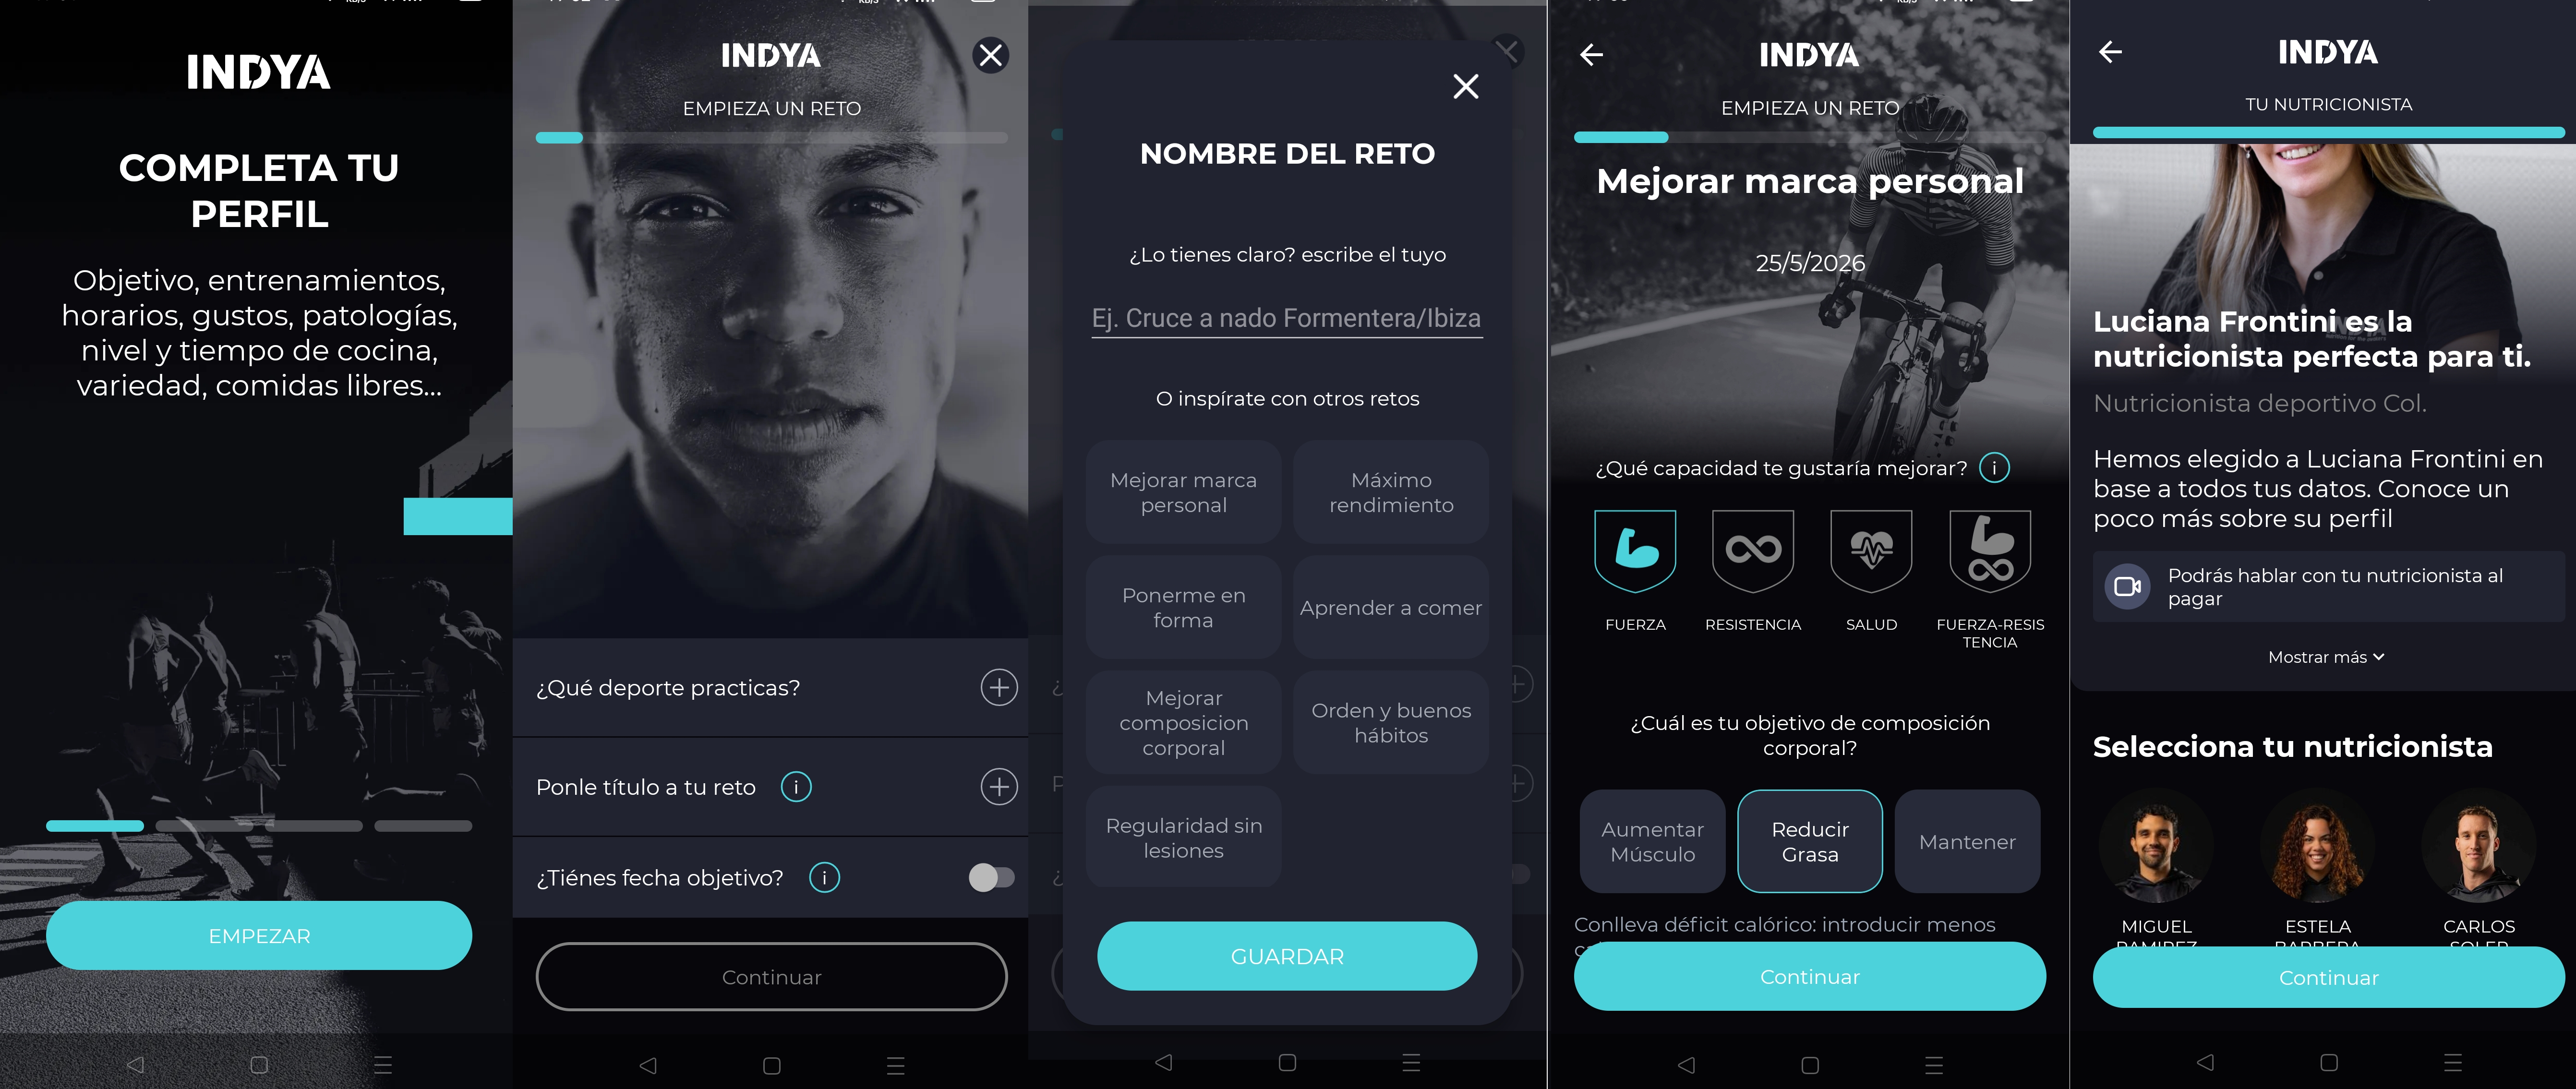
\includegraphics[width = 1\textwidth]{Imagenes/apps_images/indya.png}
	\caption{Flujo de funcionamiento de INDYA}
	\label{fig:INDYA}
\end{figure}

\section{Way of Life}

Way of Life es de entro todas las aplicaciones mencionadas, la mas sencilla pero no por ello la peor. Se trata de una aplicación simple de seguimiento de hábitos, el usuario crea un hábito y lleva un registro de cuando lo cumple y cuando no. La aplicación solo se encarga de  evaluarlo y mostrarlo gráficamente al usuario. (Ver en la figura \ref{fig:Way of Life}).

A pesar de no contar con una interfaz muy elaborada ni con unas funcionalidades apabullantes, se trata de un referente al que se aspira en el desarrollo de nuestra aplicación de hábitos saludables. Way of life combina a la perfección la sencillez con la funcionalidad al igual que HabitNow, son dos aplicaciones que ofrecen lo que prometen cuando las descargas de una forma sencilla y visual.\\

\begin{figure}[h]
	\centering
	\includegraphics[width = 1\textwidth]{Imagenes/apps_images/way_of_life.png}
	\caption{Flujo de funcionamiento de Way of Life}
	\label{fig:Way of Life}
\end{figure}

\section{Todoist}
Por último y para no hacer más hincapié en aplicaciones de gestión de tareas, tenemos Todoist. Se trata de una de las aplicaciones de gestión de objetivos y tareas más relevantes en el mercado, no solo de aplicaciones móviles, si no también de ordenadores. 

El motivo de la presencia de esta aplicación es la forma de lidiar con las tareas tan peculiar y diferente a los anteriores gestores. En este caso, Todoist abruma por su personalización y su cantidad de funcionalidades y servicios. No solo permite al usuario crear notas, permite crear las plantillas de dichas notas, algo que aumenta la experiencia del usuario.  Por ello Todoist es una herramienta muy potente  y fácil de usar. 

\section{Conclusiones}

A raíz del estudio realizado sobre diversas aplicaciones móviles disponibles en el mercado, se ha llevado a cabo un análisis centrado principalmente en herramientas de hábitos y tareas, más que en aquellas aplicaciones centradas en el control nutricional o en planes de entrenamiento para pérdida de grasa. Esto se debe a que VitHabitus, aunque tiene como objetivo final la mejora de la salud y reducción del riesgo de obesidad, el enfoque que queremos transmitir es que lo haga a través de la modificación progresiva de hábitos cotidianos y no mediante el conteo de calorías o rutinas de ejercicios. 

De esta manera, las aplicaciones analizadas Habitica, Habitify, HabitNow, Way of Life, INDYA y Todoist, han aportado una visión variada a los diferentes enfoques que se pueden tomar. 

Con este análisis se han identificado elementos positivos e imprescindibles para el desarrollo de VitHabitus como la necesidad de implementar una interfaz sencilla y amigable, evitando la sobrecarga de elementos y aumentando la simplicidad del uso de la aplicación. Por otro lado, se intenta evitar el exceso de funciones innecesarias y el uso de técnicas de enganche como premios, recompensas diarias, etc.; elementos que por el momento no se priorizan en el desarrollo.